\subsection{Позициониране чрез независими източници}

В документ \cite{bristolBeacons} се описва пасивна система, в която движещ се обект използва ултразвукови сигнали от няколко източника, за да определи позицията си в пространстовото. Движещия се обект използва разликите в периода на сигнала, което е форма на Доплеров ефект, за да определи своята позиция и скоростта си. Този подход е нов се счита за иновативен в измерването на разстоянието между различните обекти. Различава се от страндартния подход наречен time of flight (TOF), който се използва в текущата дипломна работа за измерване на разстоянията. Използвайки измервания на периода на получаване на сигнали, системата успешно идентифицира източника на даден сигнал. За да се гарантира, че приемника правилно ще идентифицира кой е текущия трансмитер, се използват подбрани периоди така че да не се получават конфликтни идентификации. За всеки трансмитер се изчислява, каква е промяната през изминалия период с помощта на зависимостта, която гласи, че изменението на пулса е пропорционално на разстоянието, което получателя е изминал през дадения период. Тази зависимост се изразява в уравнение \ref{prop}.

\centerline{\begin{equation} \label{prop}
    \Delta d = v_s \Delta P_i
\end{equation}} \\

Системата се нуждае от поне 7 трансмитера, за да работи. 

За да се определи позицията на обекта се използва Kalman филтър с множество хипотези \cite{kalmanFilter}. За да се определи позицията се ипзолзва формула \ref{kalman}.

\centerline{\begin{equation} \label{kalman}
    ((X-T_i)/ (|X-T_i|)) * V = (\Delta P_i * v_s) / (P_i + \Delta P_i)
\end{equation}}\\

Чрез изпълняванет на много паралелни филтри се генерират хипотези за позицията на обекта в пространстовото. След протичането на този процес хипотезите се комбинират. В документ \cite{bristolBeacons} е решено хипотезите да бъдат комбинирани чрез осредняване на координатите. \\


\strong{Резултати} \\
Чрез използване на Kalman филтър са измерени резултатите изобразени на фиг. \ref{fig:bristolResults}

\begin{figure}
    \centering
    \centerline{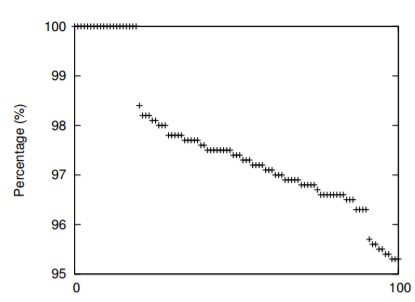
\includegraphics{bristolResults}}
    \caption{Качество на резултатите в проценти, при низходящо сортирани по дистанция данни}
    \label{fig:bristolResults}
\end{figure}